% UCL Thesis LaTeX Template
%  (c) Ian Kirker, 2014
% 
% This is a template/skeleton for PhD/MPhil/MRes theses.
%
% It uses a rather split-up file structure because this tends to
%  work well for large, complex documents.
% We suggest using one file per chapter, but you may wish to use more
%  or fewer separate files than that.
% We've also separated out various bits of configuration into their
%  own files, to keep everything neat.
% Note that the \input command just streams in whatever file you give
%  it, while the \include command adds a page break, and does some
%  extra organisation to make compilation faster. Note that you can't
%  use \include inside an \include-d file.
% We suggest using \input for settings and configuration files that
%  you always want to use, and \include for each section of content.
% If you do that, it also means you can use the \includeonly statement
%  to only compile up the section you're currently interested in.
% You might also want to put figures into their own files to be \input.

% For more information on \input and \include, see:
%  http://tex.stackexchange.com/questions/246/when-should-i-use-input-vs-include


% Formatting and binding rules for theses are here: 
%  https://www.ucl.ac.uk/students/exams-and-assessments/research-assessments/format-bind-and-submit-your-thesis-general-guidance

% This package goes first and foremost, because it checks all 
%  your syntax for mistakes and some old-fashioned LaTeX commands.
% Note that normally you should load your documentclass before 
%  packages, because some packages change behaviour based on
%  your document settings.
% Also, for those confused by the RequirePackage here vs usepackage
%  elsewhere, usepackage cannot be used before the documentclass
%  command, while RequirePackage can. That's the only functional
%  difference as far as I'm aware.
\RequirePackage[l2tabu, orthodox]{nag}


% ------ Main document class specification ------
% The draft option here prevents images being inserted,
%  and adds chunky black bars to boxes that are exceeding 
%  the page width (to show that they are).
% The oneside option can optionally be replaced by twoside if
%  you intend to print double-sided. Note that this is
%  *specifically permitted* by the UCL thesis formatting
%  guidelines.
%
% Valid options in terms of type are:
%  phd
%  mres
%  mphil
%\documentclass[12pt,phd,draft,a4paper,oneside]{ucl_thesis}
\documentclass[12pt,mphil,a4paper,oneside]{ucl_thesis}


% Package configuration:
%  LaTeX uses "packages" to add extra commands and features.
%  There are quite a few useful ones, so we've put them in a 
%   separate file.
% -------- Packages --------

% This package just gives you a quick way to dump in some sample text.
% You can remove it -- it's just here for the examples.
\usepackage{blindtext}
% This package means empty pages (pages with no text) won't get stuff
%  like chapter names at the top of the page. It's mostly cosmetic.
\usepackage{emptypage}

% The graphicx package adds the \includegraphics command,
%  which is your basic command for adding a picture.
\usepackage{graphicx}

\usepackage{subfig}

% The float package improves LaTeX's handling of floats,
%  and also adds the option to *force* LaTeX to put the float
%  HERE, with the [H] option to the float environment.
\usepackage{float}

% The amsmath package enhances the various ways of including
%  maths, including adding the align environment for aligned
%  equations.
\usepackage{amsmath}

% Use these two packages together -- they define symbols
%  for e.g. units that you can use in both text and math mode.
\usepackage{gensymb}
\usepackage{textcomp}
% You may also want the units package for making little
%  fractions for unit specifications.
%\usepackage{units}


% The setspace package lets you use 1.5-sized or double line spacing.
\usepackage{setspace}
\setstretch{1.5}

% That just does body text -- if you want to expand *everything*,
%  including footnotes and tables, use this instead:
%\renewcommand{\baselinestretch}{1.5}


% PGFPlots is either a really clunky or really good way to add graphs
%  into your document, depending on your point of view.
% There's waaaaay too much information on using this to cover here,
%  so, you might want to start here:
%   http://pgfplots.sourceforge.net/
%  or here:
%   http://pgfplots.sourceforge.net/pgfplots.pdf
%\usepackage{pgfplots}
%\pgfplotsset{compat=1.3} % <- this fixed axis labels in the version I was using

% PGFPlotsTable can help you make tables a little more easily than
%  usual in LaTeX.
% If you're going to have to paste data in a lot, I'd suggest using it.
%  You might want to start with the manual, here:
%  http://pgfplots.sourceforge.net/pgfplotstable.pdf
%\usepackage{pgfplotstable}

% These settings are also recommended for using with pgfplotstable.
%\pgfplotstableset{
%	% these columns/<colname>/.style={<options>} things define a style
%	% which applies to <colname> only.
%	empty cells with={--}, % replace empty cells with '--'
%	every head row/.style={before row=\toprule,after row=\midrule},
%	every last row/.style={after row=\bottomrule}
%}


% The mhchem package provides chemistry formula typesetting commands
%  e.g. \ce{H2O}
%\usepackage[version=3]{mhchem}

% And the chemfig package gives a weird command for adding Lewis 
%  diagrams, for e.g. organic molecules
%\usepackage{chemfig}

% The linenumbers command from the lineno package adds line numbers
%  alongside your text that can be useful for discussing edits 
%  in drafts.
% Remove or comment out the command for proper versions.
%\usepackage[modulo]{lineno}
% \linenumbers 


% Alternatively, you can use the ifdraft package to let you add
%  commands that will only be used in draft versions
%\usepackage{ifdraft}

% For example, the following adds a watermark if the draft mode is on.
%\ifdraft{
%  \usepackage{draftwatermark}
%  \SetWatermarkText{\shortstack{\textsc{Draft Mode}\\ \strut \\ \strut \\ \strut}}
%  \SetWatermarkScale{0.5}
%  \SetWatermarkAngle{90}
%}


% The multirow package adds the option to make cells span 
%  rows in tables.
\usepackage{multirow}


% Subfig allows you to create figures within figures, to, for example,
%  make a single figure with 4 individually labeled and referenceable
%  sub-figures.
% It's quite fiddly to use, so check the documentation.
%\usepackage{subfig}

% The natbib package allows book-type citations commonly used in
%  longer works, and less commonly in science articles (IME).
% e.g. (Saucer et al., 1993) rather than [1]
% More details are here: http://merkel.zoneo.net/Latex/natbib.php
%\usepackage{natbib}

% The bibentry package (along with the \nobibliography* command)
%  allows putting full reference lines inline.
%  See: 
%   http://tex.stackexchange.com/questions/2905/how-can-i-list-references-from-bibtex-file-in-line-with-commentary
\usepackage{bibentry} 

% The isorot package allows you to put things sideways 
%  (or indeed, at any angle) on a page.
% This can be useful for wide graphs or other figures.
%\usepackage{isorot}

% The caption package adds more options for caption formatting.
% This set-up makes hanging labels, makes the caption text smaller
%  than the body text, and makes the label bold.
% Highly recommended.
\usepackage[format=hang,font=small,labelfont=bf]{caption}

% If you're getting into defining your own commands, you might want
%  to check out the etoolbox package -- it defines a few commands
%  that can make it easier to make commands robust.
\usepackage{etoolbox}

% Include Acronym glossary 

\usepackage[nopostdot,% remove dot after description
  indexonlyfirst,% only index first use
  nomain,acronym,xindy,numberline]{glossaries}
%\makeglossaries 




% Sets up links within your document, for e.g. contents page entries
%  and references, and also PDF metadata.
% You should edit this!
\input{LinksAndMetadata}

% And then some settings in separate files.
\input{FloatSettings} % For things like figures and tables
\bibliographystyle{apalike}   % For bibliographies

% These control how many number sections your subsections will take
%    e.g. Section 2.3.1.5.6.3
%  and how many of those will get put into the contents pages.
\setcounter{secnumdepth}{3}
\setcounter{tocdepth}{3}

\makeglossaries

\newacronym{SPECT}{SPECT}{Single Photon Emission Computed Tomography}

\newacronym{CT}{CT}{Computed Tomography}

\newacronym{MRI}{MRI}{Magnetic Resonance Imaging}

\newacronym{MR}{MR}{Magnetic Resonance}

\newacronym{PET}{PET}{Positron Emission Tomography}

\newacronym{PET/MR}{PET/MR}{Positron Emission Tomography/ Magnetic Resonance}

\newacronym{PET/MRI}{PET/MRI}{Positron Emission Tomography/ Magnetic Resonance Imaging}


\newacronym{PET/CT}{PET/CT}{Positron Emission Tomography/ Computed Tomography}

\newacronym{SPECT/CT}{SPECT/CT}{Single Photon Emission Computed Tomography/ Computed Tomography}

\newacronym{SPECT/MR}{SPECT/MR}{Single Photon Emission Computed Tomography/ Magnetic Resonance}

\newacronym{SPECT/MRI}{SPECT/MRI}{Single Photon Emission Computed Tomography/ Magnetic Resonance Imaging}

\newacronym{INSERT}{INSERT}{ Integrated SPECT/MRI for Enhanced Stratification in Radio-chemotherapy}

\newacronym{FOV}{FOV}{Field of View}

\newacronym{ML}{ML}{Maximum Likelihood}

\newacronym{MLEM}{MLEM}{Maximum Likelihood Estimation Maximisation}

\newacronym{COM}{CoM}{Centre of Mass}

\newacronym{MSS}{MSS}{Multi-mini-slit Slit-Slat}

\newacronym{PMT}{PMT}{Photomultiplier Tube}

\newacronym{simpm}{SiPM}{Silicon Photomultiplier}

\newacronym{DOI}{DOI}{Depth of Interaction}

\newacronym{LRF}{LRF}{Light Response Function}

\newacronym{FWHM}{FWHM}{Full Width Half Maximum}

\newacronym{CFOV}{CFOV}{Central Field of View}

\newacronym{UFOV}{UFOV}{Useful Field of View}

\newacronym{COV}{CoV}{Coefficient of Variation}

\newacronym{UCL}{UCL}{University College London}

\newacronym{UCH}{UCH}{University College Hospital}

\newacronym{HSR}{HSR}{San Raffaele Hospital}

\newacronym{NEMA}{NEMA}{National Electrical Manufacturers Association}

\begin{document}

\nobibliography*
% ^-- This is a dumb trick that works with the bibentry package to let
%  you put bibliography entries whereever you like.
% I used this to put references to papers a chapter's work was 
%  published in at the end of that chapter.
% For more information, see: http://stefaanlippens.net/bibentry

% If you haven't finished making your full BibTex file yet, you
%  might find this useful -- it'll just replace all your
%  citations with little superscript notes.
% Uncomment to use.
%\renewcommand{\cite}[1]{\emph{\textsuperscript{[#1]}}}

% At last, content! Remember filenames are case-sensitive and 
%  *must not* include spaces.
% I may change the way this is done in a future version, 
%  but given that some people needed it, if you need a different degree title 
%  (e.g. Master of Science, Master in Science, Master of Arts, etc)
%  uncomment the following 3 lines and set as appropriate (this *has* to be before \maketitle)
% \makeatletter
% \renewcommand {\@degree@string} {Master of Things}
% \makeatother

\title{A Thesis Title}
\author{Ashley James Morahan}
\department{Department of Medical Physics and Biomedical Engineering}

\maketitle
\makedeclaration

\begin{abstract} % 300 word limit
The aim of this project was to assess the performance of a novel Single Photon Emission Computed Tomography system (SPECT); designed to be compatible with Magnetic Resonance Imaging (MRI). The SPECT insert is the first clinical system of its kind, aiming to improve patient treatment and perform simultaneous scanning of the brain. The system has been created in a simulation and testing of its design was carried out. A series of experiments were designed using different system geometry, phantoms and photon energy. The aims of these experiments were to evaluate the system performance under a number of conditions, pushing the system past the functional environment it was designed for.
\paragraph{}
The novel system required thorough testing in order to validate its design specifications and quantify its performance. A focus of the testing was to determine the extent of septal penetration through the novel collimator design. We aimed to measure this phenomenon and use a model to quantify its effects on the system. Through this result we hoped to determine the limits of the system and to improve the design. Another focus was to measure the depth of interaction of high energy photons. The result of this measurement could improve the image reconstruction algorithm, allowing for higher quality clinical images to be produced.
\paragraph{}
The results of the simulated experiments helped to determine the limits of the systems performance. Analysing the system built an understanding of the novel design and can help to improve the system. The information gained from these experiments can be used to improve the design and work towards a fully operational dual-imaging system.
\paragraph{}
The development of the first clinical simultaneous Single Photon Emission Computed Tomography (SPECT) and Magnetic Resonance Imaging (MRI) system was carried out within the INSERT project. The INSERT scanner was constructed under the initial project but its performance was not fully evaluated; here we have reconstructed the first images on the SPECT system. Calibration and acquisition protocols were developed and used to establish the clinical feasibility of the system. The image reconstruction procedures were implemented on the first phantom images in order to assess the system's imaging capabilities. This study solved issues involving incomplete data sets and pixel failure in the prototype detector system. The final images determined a measure of trans-axial image resolution, giving average values of 9.14 mm and 6.75 mm in the radial and tangential directions respectively. The work carried out on the complete system produced a number of clinical phantom images which utilised the capabilities of both SPECT and MRI.
\end{abstract}

\begin{impactstatement}

\end{impactstatement}


\begin{acknowledgements}
I acknowledge the use of image reconstruction provided by Dr. Kjell Erlandsson, \cite{8069508}.
\paragraph{}
I would like to thank Professor Brian Hutton and Dr. Kjell Erlandsson for providing their advice and supervision in this project. 
\paragraph{}
Thank you to the team at INM and the UCL i4Health for all their support. 
\end{acknowledgements}

\setcounter{tocdepth}{2} 
% Setting this higher means you get contents entries for
%  more minor section headers.

\tableofcontents
\listoffigures
 \listoftables
%\newacronym{spect}{SPECT}{Single Photon Emission Computed Tomography}

\newacronym{mri}{MRI}{Magnetic Resonance Imaging}
\printglossaries

\chapter{Introductory Material}
\label{Introduction}
% discuss SPECT and Multimodal 
% SPECT 
% Photon Detection (and collimation)
% Event reconstruction .Recon techniques pg51 Mic.
%Image Recon 
% Calibration Techniques Deb Pg. 49 

This thesis outlines the evaluation of a \acrshort{SPECT} imaging system, designed for the simultaneous use within a clinical \acrshort{MRI} system. This chapter outlines the basics of \acrshort{SPECT} imaging systems, discusses the use of multi-modality imaging and introduces the novel combined imaging system; the \acrshort{INSERT} scanner. 

\section{SPECT}
The \acrlong{SPECT} system was introduced by \cite{Anger} as a method of retrieving a signal from the detection of gamma photons. \acrshort{SPECT} is used widely as a medical imaging technology to investigate the physiological response of an injected radio-pharmaceutical. A pharmaceutical is chosen by its ability to target a given biological process or organ, this drug is labelled with a gamma emitter. The localised emission is detected by the \acrshort{SPECT} camera and the resulting signal is reconstructed into a 3D tomographic image. The main components of the \acrshort{SPECT} developed by \cite{Anger and Rosenthal} are the collimator, scintillation crystals and \acrlong{PMT}. The gamma rays emitted from the patient will travel toward the camera head; they interact with the scintillation crystal producing a light pulse, the \acrshort{PMT} will amplify this pulse and convert it to an electrical signal for processing. The signals are processed using Anger logic, \cite{angerLogic}, however without a geometric context it is impossible to localise the origin of the gamma ray; the collimator acts as a camera aperture by allowing only gamma rays from a chosen direction to enter the crystal.

Photon detection within a \acrshort{SPECT} is governed by many factors. The collimator design is the largest contribution to sensitivity, resolution and \acrlong{FOV} of the system. The choice of collimator must consider a balance between number of photons detected and the quality of localisation. A high resolution will improve localisation but is achieved by reducing the aperture size; reducing the sensitivity and requiring a longer scanning time. The collimator is also chosen with consideration of the desired image; for example collimator designs such as the pinhole are more suited to small organ imaging. The geometry of the collimator determines how the acquired signal is processed into a final image. The chosen collimator geometry defines the photon path however there are uncertainties to consider such as photons penetrating through the collimator septa. 

The localisation of photons is also determined by the design of the scintillation crystals and \acrshort{PMT}. These components determine performance factors of the detector including efficiency, count rate, spatial and energy resolutions, uniformity, and linearity. The size, position and density of the crystal determines the efficiency of photon detection. A greater efficiency improves the count rate as event are not lost in between scintillation interactions due to dead time. The energy resolution is the detectors ability to distinguish the photopeaks within a spectra. The spatial resolution of a detector defines the quality of spatial information for each event, this is governed by the \acrshort{PMT} geometry and the photons \acrlong{DOI} within the crystal. Uniformity and linearity are important factors in image quality as the spatial response may be unstable depending on time or location.

\section{SPECT Imaging} % Reword
\acrshort{SPECT} imaging systems determine the location of a radioactive tracer within the body from the forward projection of the acquired data. The process of imaging is governed by the solution of the equation \ref{eqn:imgRec}. The value of $x$, the tracer activity, is determined from the acquired data, $Y$, and the system matrix, $S$; subject to a noise term, $\eta$. The solution give a complete image of the object by acquiring projections from several angles. More information from the object is acquired with each addition projection angle. We extract the tracer information from a sinogram; a representation of projection data moving through all covered angles. The reconstructed images are produced through the analytical or iterative solution of \ref{eqn:imgRec}. The projections are created using event reconstruction algorithms. These are based on Anger logic; this thesis focuses on two methods of event reconstruction used to evaluate the projection data acquired from each experiment.

\begin{equation} \label{eqn:imgRec}
        Y = S(X) + \eta 
\end{equation}

\subsection{Event Reconstruction: Centroid Method}
The \acrlong{COM} method, also known as the Centroid method, is a simple reconstruction originating in the first Anger cameras. From Anger logic we know the signal from a scintillation event will decrease further from the interaction point. The Centroid algorithm makes use of this by simply considering a weighted mean of the signal of a given event from each photodetector. 

\begin{equation} \label{eqn:Centroid}
        X_{i} = \frac{\sum^{N}_{j} x_{j} \cdot S_{ij}}{\sum^{N}_{j} S_{ij}} \quad ; \quad  Y_{j} = \frac{\sum^{N}_{j} y_{j} \cdot S_{ij}}{\sum^{N}_{i} S_{ij}}
\end{equation}

The equation \ref{eqn:Centroid} describes the reconstructed event positions $X\_i$ and $Y\_i$ for each event i. The signal $S\_{ij}$ from a given event is summed over each  photodetector j. This weighted sum gives the likely position of an event as the coordinates is calculated toward the centre of the nearest photodetecto, $x\_j$ and $y\_j$. The centroid method is modified to account for the event compression towards the centre of a given detector; this modified centroid method subtracts a common baseline, B, value from each event. The baseline subtraction removes signal not within the region of interest and is chosen based on the detectors field of view (\ref{eqn:ModCent}). 

\begin{equation} \label{eqn:ModCent}
        X_{i} = \frac{\sum^{N}_{j} x_{j} \cdot (S_{ij} - B)}{\sum^{N}_{j} S_{ij}} \quad ; \quad  Y_{j} = \frac{\sum^{N}_{j} y_{j} \cdot (S_{ij} - B)}{\sum^{N}_{i} S_{ij}}
\end{equation}

This method is popular as is provides fast and simple projection data. Although the baseline solves the central compression, the centroid method is subject to several errors. 

Non-uniformity in a given camera will distort the resulting projection. Uniformity and sensitivity are subject to the detector response to relative gain and energy window selection. The difference between photodetectors gain can result in false density distribution across the whole detector. The centroid method is unable to account for this as signal will be heavily weighted by a non-uniform photodetector. 

Linearity of the projection data is subject to spatial distortion within the crystal, the centroid method assumes a constant response throughout the crystal. Although true for the centre of the crystal this assumption results in non-linearity at the detector edges. The result is similar to the central compression from equation \ref{eqn:Centroid}.

These issues can be resolved with correction maps as we will see in the following chapters. However we can improve the event reconstruction through statistical methods and spatial modelling. 

\subsection{Event Reconstruction: Maximum Likelihood}
A statistical method of event reconstruction is able  to produce higher quality projection data which is less susceptible to spatial distortions. The \acrlong{ML} algorithm achieves this by accounting for the random nature of gamma particle interactions and extracting probability models from acquired data.

The \acrshort{ML} algorithm makes use of optical models and the detectors spatial response to calculate the events coordinates and energy. The algorithm optimises a set of model parameters in order to maximise the probability of observing the acquired data from the given model. If we consider our observed data by vector $\Bar{\nu}$, each value is given by detector response to a scintillation event, i.e. number of detected photons or electrical signal, by each channel. The observed data is a result of a series of random events, $V\_i$ (in SPECT imaging this is the transport of gamma rays). The events can be represented by a known probability model, $M(\theta)$, where $\theta$ is the set of optimising parameters. Thus the probability of observing our acquired data given $\theta$ is the joint probability of each independent event $V\_i$ for N total events. 

\begin{equation} \label{eqn:MLProb}
                P(\Bar{\nu}|\theta) = \prod^{N}_{i=i}P(V_i)
\end{equation}

The likelihood of the observed sample, $L(\theta|\Bar{\nu}) = P(\Bar{\nu}|\theta)$, can be maximised to retrieve the unknown parameter which gives the observed data. The standard form for the \acrshort{ML} algorithm takes the log of the maximisation to turn the product into a sum. 

\begin{equation} \label{eqn:ML}
                \hat{\theta} = max\{\sum^{N}_{i=i}log(L(\theta|\Bar{\nu}))\}
\end{equation}


\subsection{Image Reconstruction}
Once the projection data has been reconstructed the final images can be produced from the solution to equation \ref{eqn:imgRec}. Here we briefly describe the iterative approach which is used throughout this thesis. The \acrlong{MLEM} algorithm aims to produce a image model which accounts for the physical interactions involved in \acrshort{SPECT} imaging; optimising the model until it matches the acquired data, \cite{4307558}. Using the \acrshort{ML} logic described above the algorithm carries out a series of forwards and back projections in order to improve a estimated model. The algorithm is composed of two main steps; the estimation stage, and the maximisation stage. The initial estimation can be a uniform image or can be retrieved from a simple back projection of the acquisition data. The estimated model is forward projected to produce a model of the measured projection data. The projection models are then compared with the acquired data. A correction term is derived from this comparison; using the maximum likelihood technique a correction is determined and used to improve out estimation. This is the maximisation step, the result is an improved image when back projection is carried on on the estimation. However this improvement is incremental and so the steps must be repeated; improving the model and creating a image closer to the true object with each iteration.  

\section{Multi-modal Imaging} % dont discuss INSERT 
% Multi modal 
The capabilities of medical imaging continues to improve and expand, however in recent years it has become possible to combine medical imaging systems. Multimodal imaging technologies have gained popularity within research and clinical practice for their ability to simultaneously or sequentially acquire data from multiple systems. Individual systems can provide either functional or structural information, however many patients require multiple scans for diagnosis or treatment. The combination of this information is essential in investigations and can be achieved through methods such as spatial and time registration. However, acquiring multiple scans and registering the images takes many hours and is subject to errors such motion. Multimodal systems can solve this by acquiring both structural and functional information within one simultaneous scan, reducing scan time and improving image registration. 

Mulitmodal systems such as \acrlong{SPECT/CT} and \acrlong{PET/MRI} have been widely implemented in the clinic as they combine anatomical information from the \acrshort{CT} and \acrshort{MR}, with the biochemical or metabolic information of \acrshort{SPECT} and \acrshort{PET}. The combination of these systems is achieved through the development of innovative technologies and designs, as well as the improved computational methods. This can prove expensive and challenging as individual systems may not be compatible. \acrshort{PET/MRI} was achieved through the development of \acrshort{MR} compatible detectors. \acrshort{PET/MR} and \acrshort{SPECT/CT} have been highly successful in the clinic as it produces combined structural and functional images. 

However a sequential \acrshort{SPECT/MRI} clinical system has yet to be established. The combination of \acrshort{SPECT} and \acrshort{MRI} can be carried out through sequential use of \acrshort{SPECT/CT} and \acrshort{MRI}. The data are registered to provide the \acrshort{SPECT/MR} images useful in areas should as tumour treatment planning. In the case of \acrshort{SPECT/CT}, the radiation \acrshort{CT} introduces additional dose and the acquisition is not as versatile of \acrshort{MRI}. The development of simultaneous and integrated \acrshort{SPECT/MRI} promises the advantages of \acrshort{PET/MR}. \acrshort{MRI} has proven a powerful and versatile imaging method, providing greater diagnostic information with no dose. \acrshort{SPECT} imaging is more widely available and cheaper than \acrshort{PET} systems; \acrshort{SPECT} is popular as it allows the use of more accessible radionuclides and dual-isotope imaging.

It stands to reason that a simulataneous clinical \acrshort{SPECT/MR} system could provide a multifaceted imaging tool. This thesis outlines the use of the\acrshort{INSERT} scanner; the first clinical simultaneous \acrshort{SPECT/MRI} imaging system. The goal of which is to provide brain tumour imaging and treatment stratification, and establish a foundation of a completely integrated \acrshort{SPECT/MRI} system. 

\begin{figure}[htp]
    \centering
    \includegraphics[width=0.9\textwidth,keepaspectratio]{INSERT_design} % name of file without extension
    \caption{The design for the partial ring INSERT system.} \label{fig:INSERT}
\end{figure}

 % Multimodal and tech 
\chapter{INSERT}
\label{chapterlabel2}
% general system design
% Detection module 
% collimator
% Hardware evaluation/ PSMR paper 
% Current state (Milan experiments and London installation)

As stated in the introduction the INSERT project aims to incorporate a SPECT module insert into existing MRI devices. The device will fit into the MRI bore and carry out a simultaneous SPECT and MRI scan of the brain. The challenges faced in this design arise from the need a compact, MR compatible SPECT system.
\section{Compatibility and Design}
The traditional SPECT design makes use of a collimator, scintillation crystals and PMT's to acquire a signal. The use of SPECT in an MR environment requires components which are able to function in the presence of a strong magnetic field. In order for simultaneous acquisition the SPECT design must be compact and fit within the MRI bore. To fit these requirements, the INSERT is designed with MR compatible photon detection \cite{7287793} and a novel collimator design \cite{7181734}. As stated previously the PMT is incompatible with the requirements for the INSERT system. 
\paragraph{}
It is essential that the SPECT device does not include any materials which are MR incompatible. Magnetic materials must not be present in the SPECT unit. The varying magnetic fields may also induce eddy currents in some metals. These currents can reduce the performance by introducing their own magnetic fields which are detected by the MR coils. 
\paragraph{}
The SPECT system must acquire the image data through stationary means. The SPECT unit must not move as motion will cause artefacts in the MRI acquisition. The stationary system will have to collect the information from all angles with a ring of detectors. This furthers the need for a compact system. To ensure there is room for the patient the bed, the scanner is designed with a partial ring structure.
\section{Photon Detection}
The INSERT must make use of methods of photon detection without the PMT. This can be achieved through MR compatible solid state devices. The device chosen in the INSERT design is the Silicon Photomultiplier (SiPM), this is a compact solid state device which is able to function within a strong magnetic field, \cite{SCHAART201631}, \cite{0031-9155-56-23-014}. SiPM are formed of thousands of Avalanche Photodiode (APD), functioning in Geiger mode (G-APD). An APD is able to produce a large output current (avalanche current) from even a single charge carrier input, similar to the PMT, however these solid state devices pass carriers through a bulk material such as silicon as opposed to the vacuum used in PMTs, \cite{RENKER200648}. G-APDs consist of a reverse biased PN junction. The PN junction is a boundary composed of a pair of semiconductor materials, known as the P and N type materials. The materials are doped to produce a positive (P type) or negative (N type) region, these define the valence and conductive bands in the semiconductor. When a reverse bias is applied a high resistance junction is created as the band gap increases. The avalanche current is caused by the break down of the high resistance junction as electron hole pairs are produced. A single electron with sufficiently high kinetic energy can ionise the silicon and the resulting pair will travel to opposing bands liberating further electrons and hole, leading to the avalanche. However this design has an intrinsic limitation in which the output is unable to distinguish input magnitude.
\paragraph{}
A SiPM is composed in a microcells, a series of SiPM arranged together each generating a combined G-APD avalanche signal, \cite{DINU2015367}. This design overcomes the G-APD limitation as the microcells produce individual localised signals, which give an output proportional to the activation of the microcells. The SiPM are arranged in a minimally spaced array to cover the detector surface with maximum light detection. The SiPM requires a cooling unit to maintain a functioning temperature. The SiPM is optimised to detect the wavelength from the chosen scintillation crystal. A Thallium activated Cesium Iodide (CsI(Tl)) crystal is used for the scintillation of photons. This inorganic crystal was chosen for its high output signal despite its slow performance. The crystal is 8 mm thick and the total thickness of the SiPM with cooling unit and required electronics is 21.69 mm. This thickness is much smaller than the PMT design, and fits in the MRI bore. The crystal and SiPM define an intrinsic resolution of 1 mm for the detector system.
\section{Collimator}
The novel collimator unit is essential to the design of the INSERT project. The collimator is designed to account for the size and stationary requirements of the system, constructing a partial ring which aims to maximise sensitivity and reduce dead space. The collimator design chosen is a Multi-Slits Slit Slat (MSS) collimator. This collimator provides a compact design to satisfy the space requirements. The coverage of the collimator must be maximised to account for the limitations in angle coverage from a stationary system. To acquire the desired functional information the sensitivity is also maximised by this coverage design. Figure \ref{fig:MSSColl} demonstrates the design of the MSS collimator. The slits are separated by a sections of two and three slits, with slats across each slit.

\begin{figure}[htp]
    \centering
    \includegraphics[width=0.8\textwidth,keepaspectratio]{Collimator_schema} % name of file without extension
    \caption{The MSS collimator deisign schematic show blue slits with red slats. Figure from \cite{8069508}} \label{fig:MSSColl}
\end{figure}

\paragraph{}
The collimator consists of a series of slits which run along the length of the collimator in alternating pairs and triplets, these are labelled the `2 slits' and the `$1 + 2\frac{1}{2}$ slits'. The furthest edge `$2\frac{1}{2}$ slits'  combine with those of the neighbouring collimator to cover a wider angular range across the ring. The field of view (FOV) covered by the slits in the trans-axial plane is 20 cm. The large FOV is a result of the radially position slits and fanned out individual slits. The small system design leads to minification of the object in the the trans-axial plane, within the FOV. The resolution and sensitivity of the slit is given by the pin hole equations (\ref{eqn:pinholeRes},\ref{eqn:pinholeSen}).
\paragraph{}
The collimator has a series of parallel slats running perpendicularly all along the length of the slits. These slats define the resolution in the axial direction. The parallel hole equations (\ref{eqn:ParholeRes},\ref{eqn:ParholeSen}) define the resolution and sensitivity of the parallel slats. The axial FOV is 9 cm and induces no minification in this direction. Together the slits and slats define a cylindrical field of view. The slits carry out pin hole collimation and have a fan beam acceptance angle, where the slats have a parallel beam range. The design is expected to give a resolution of 8 - 10 mm within the FOV. The resolutions of the slit and slats can be considered separately  as they span different planes, however the overall sensitivity of the system must be some combination of the slit and slat apertures. Metzler \cite{Metzler2010SlitSlatAM} demonstrates the sensitivity equation derived from this kind of equation.
\paragraph{} 
To ensure MR compatibility the collimator must be constructed with a material which does not induce eddy currents, \cite{7286864}. The MSS collimator is constructed with tungsten in order to reduce the effects of eddy currents. Tungsten has a high stopping power however it is brittle, requiring a certain thickness for practical purposes. The collimator septa spacing defines the spatial resolution, this resolution is great limitation in SPECT imaging. The collimator design must balance the trade off between resolution and sensitivity whilst also considering the functionality and shielding, more on this in the next chapter. The shielding of the camera had to consider the practical aspect of device weight. In order to reduce the weight of the collimator the internal material was cut down. This reduced the shielding capabilities but was done so as to keep within the minimum accepted penetration. 


\begin{equation} \label{eqn:pinholeRes}
        R_{pinhole} = \frac{\omega(h + f)}{f}
\end{equation}


\begin{equation} \label{eqn:pinholeSen}
        g_{pinhole} = \frac{\omega \cos^{3}(\theta)}{16h^{2}}
\end{equation}

\begin{equation} \label{eqn:ParholeRes}
        R_{\parallel} = \frac{d(l + z)}{l}
\end{equation}


\begin{equation} \label{eqn:ParholeSen}
        g_{\parallel} = \frac{d^{4}}{12l^{2}(d+t)^{2}}
\end{equation}
 % Hardware and project so far inc installation 
%\chapter{Event Reconstruction}
\label{chapterlabel}
% software (PERA pg 137 Deb. 65 Il.)


\section{Introduction}
Following the initial results of the linearity correction software; the event reconstruction protocol of the system was revisited to  establish how we can improve the quality of the projection data. The event reconstruction makes use of both centroid and ML reconstruction algorithms. 
\section{Methods}
The event reconstruction is initialised with the centroid reconstruction, making use of a minimum count baseline to remove scatter events. This initial reconstruction is used by the ML algorithm to establish a final projection image. The ML models the detectors spatial response with the LRF of each SiPM individually. The hardware issues lead to a failure in the LRF as faulty channels were not modelled correctly. A solution to this would be to create a new LRF for the faulty detector, however the LRF take a long time to produce; we proposed a normalised LRF approach for more adaptable modelling. The list-mode data was normalised with respect to the mean counts in order to reduce the effect of anomalous events. The LRF and centroid projections were produced using the normalised LM. This ensured they matched and would account for hot spots or faulty channels in the data.
\section{Results}

\section{Discussion}

\section{Conclusion} % PERA method and new 
\chapter{Experiments 01}
\label{Milan}


% Evaluation method and calibration 
% Detector Cal 
% System Cal 
% System evaluation 
% hard ware issues 

% New Event Recon (killed_LRF, FilteredSpectrum, Normalisation)
% New Linearity software (3 methods) 
In this chapter the use of the \acrshort{INSERT} scanner is outlined. The calibration procedures and experimental methods explored in this chapter are used to evaluated the system performance. The outcome of this investigation resulted in the implementation of new data processing methods. 

\section{Introduction}
The following experiments were carried out at San Raffaele Hospital (Milan), in collaboration with Politecnico di Milano (POLIMI). The system was transported and installed in the nuclear medicine department in order to carry out experiments with radioisotopes such as Technetium-99m. The experiments were carried out using the BULMA software provided by Mediso Ltd (Budapest). The software was designed to operate the system and acquired the raw data from experiments. The raw data was processed and calibrated using the BULMA INSERT-GUI package along with existing system data. 

This experiments set out to acquire the first phantom images from the \acrshort{INSERT} system, in order to achieve this the system was first evaluated and calibrated. The count-rate and energy resolution were determined and the system corrections and calibrations for these parameters where carried out at Polimi. The calibration procedures required to correct for event and image reconstruction are outlined here.

The calibration procedure was developed on a single detector head system \cite{DebCal}, and was tested in this investigation for the first time on the complete \acrshort{INSERT} scanner. This investigation aimed to determine the effectiveness of the proposed calibration method, and evaluate the systems performance and imaging capabilities. The calibration involves two stages, the detector calibration and the system calibration. The event reconstruction was corrected through the detector calibration procedure; a standard linearity and uniformity correction was performed. The image reconstruction was carried out using the geometric and sensitivity information obtained by the system calibration.

%\section{Methods}
\section{Detector Calibration}
The detector calibration is carried out by collecting uniformity and linearity data from each detector head. The uniformity of a given detector head is determined by the intensity variation across a planar acquisition. The uniformity is subject to spatial variations in the crystal properties such as, stopping power and number of emitted scintillation photons. Linearity is a measure of location dependent spatial distortion. This measured by reproducing a known linear geometry. Both uniformity and linearity are subject to position and time variations and so we must calibrate each detector regularly.

The uniformity data is collected by performing a flood scan of a single point source (1 MBq of $^{99m}Tc$) located in the centre of the scanner \acrshort{FOV}. The uniformity scan was carried out without the collimator attached; consequently short scans are required due to the high counts. The uniformity scans were collected once and used to correct for uniformity in the subsequent phantom acquisitions. 

The linearity distortion in a given detector was measured by acquiring data from a planar phantom (4 MBq of $^{99m}Tc$) mounted a set of parallel line collimators. Two collimator scans are carried out on each head; measuring the distortion in the X and Y direction respectively. The phantom attached of linearity collimator covered the whole detector head and so each unit was scanned individually. 40, 4 minute scans were required to collect the complete set of X and Y linearity data. 

\subsection{Detector Calibration Software}
The resulting data is processed using the BULMA software. The uniformity and linearity data is used to produce a set of transformation maps which are applied during the planar event reconstruction. As discussed previously the planar event reconstruction is carried out in a two step method; a centroid reconstruction is used to initialise an \acrshort{ML} reconstruction. Part of the \acrshort{ML} algorithm is the modelling of the detectors spatial response, the aforementioned \acrshort{LRF}. The BULMA software included existing \acrshort{LRF} data for the system, however it was found that this data was incorrect for the current system. The uniformity flood was used to produce a new set of \acrshort{LRF} models, which were incorporated in the event reconstruction.

The \acrshort{LRF}, uniformity, and the X/Y linearity data are input into the BULMA software alongside the raw uncorrected phantom data. The X and Y data are firstly reconstructed to produce two planar images of linear bands. The software uses active contour splines to identify the data bands. The resulting X and Y splines are combined to produce a grid of crossing control points; the linearity map is created. The photopeak of the total phantom data is determined and an initial reconstruction is found using the \acrshort{LRF}. The linearity map crossing points mark out positions to determine the local energy spectra; these produce a local, position-dependent, energy filter. The energy at each pixel position in the phantom reconstruction are calculated and matched to the local energy map. Correcting for the local energy peaks produces a planar reconstruction corrected for energy and linearity. The uniformity data is reconstructed in the same way to create the uniformity map. The phantom reconstruction is multiplied by the inverse of the uniformity map to correct each pixel. The final result is corrected planar image, ready for image reconstruction. 

%\subsection{Uniformity}
%\subsection{Linearity} 

\section{System Calibration}
The image reconstruction algorithm requires information of the systems geometry and sensitivity. The system calibration acquires this information through two experiments. Each experiment is carried out with the collimator fitted. The data from each experiment produces correction which are applied to the planar images during image reconstruction. 
 
The geometric calibration has been established previously, \cite{8340862}. The geometric data is acquired from a series of scans of capillary phantoms. The capillaries have 1 mm diameter and are filled with 10 MBq of $^{99m}Tc$. Two experiments are set up to acquire the axial and trans-axial geometry of the system. 

\textbf{Axial Orientation:} The capillaries were aligned with the axial direction of the scanner. The capillaries are held on a rotating stage and positioned at 4 locations with the \acrshort{FOV}. The positions are separated by $90\degree$ and lie at radii of 25, 50, 75 and 100 mm. From these positions the capillaries are rotated about the z axes of the scanner. The capillaries are scanned for 2 minutes at 30 positions; rotating by $12\degree$ until $360\degree$ is covered. 

\textbf{Trans-axial Orientation:} similarly the capillaries were placed along the trans-axial plane and rotated about the z axes. Five capillaries are at positions, $ 0, \pm 5, \pm 10 $ cm from the centre of the bore. Due to time constraints these capillaries were only scanned for 5 positions.

The sensitivity calibration required data with a planar phantom, $10 * 10 * 0.5$ cm, filled with 50 MBq of $^{99m}Tc$. The phantom was place in front of each detector head and scanned individually. The phantom covered the whole collimator \acrshort{FOV}, the resulting flood acquisition gave a measure of uniformity variation due to the collimator geometry. 

\subsection{System Calibration Software}
The data collected from the system calibration undergoes planar event reconstruction and detector calibration as described above. The resulting data was analysed in MATLAB.

The geometric data was used to measure 3 system parameters of the collimator. The tilt and twist angles, and mechanical shifts were determined by modelling the variation in position and size of the capillary data. The location of each capillaries is measures with a Gaussian model by taking measurements along its length. The variation in position as a function of radial position of the axial capillaries is known as the mechanical shift in the collimator. The variation of position along the length of a trans-axial capillary is known as the twist angle. Finally the variation in position as a function of radial position of the trans-axial capillaries gives us a measure of the tilt angle. 

The reconstructed sensitivity profiles gave a measure of count variation across the whole collimator. The sensitivity variation as a function of sampling angle of the aperture was modelled. Each profile was fitted using equation (\ref{sens_model}), where $\phi$ is the sampling angle, $G_{\sigma}(\phi)$ is a Gaussian function. The summation is carried out over all mini-slits $i$ for each collimator section $j$. The model is used to correct for sensitivity variation in the planar projection data. 

\begin{equation}
%\vspace{-0.2cm}
\label{sens_model}
S_{j}(\phi) = \sum_{i} G_{\sigma}(\phi) \ast A_{i,j} \cos^{p}{\phi} + b_{j}(\phi)
%\vspace{-0.2cm}
\end{equation}

\section{Results}
The calibration procedures were used to carry out the correct image reconstruction of the phantom data, the use of this data will be shown in chapter \ref{IEEE}. However, the data collected in these experiments were also used to assess the system performance and to determine system properties such as resolution and stability. 

\subsection{Detector Calibration}
 The uniformity scans were used to quickly assess the condition of each detector. The initial assessment revealed the presence of faulty channels in some detector heads. A faulty channel would produce a high number of false counts which resulted in a hot spot; drowning out the healthy channels and giving further false counts to neighbouring channels. The solution to this was to turn off, or 'kill', the offending channels and leave a single dead channel in its place. The dead channel left a large gap in the projection data; event reconstruction was carried out but detector calibration was not possible. The \acrshort{LRF} provided a solution to this problem as it gave the spatial response for each individual channel. The killed channels were therefore modelled as a such in the \acrshort{LRF} data. This was achieved by building an \acrshort{LRF} model with the 'killed' uniformity data. This allowed the \acrshort{MLEM} reconstruction to model the missing data and interpolate events from neighbouring channels. The modified reconstruction significantly reduced the data gap left by the faulty channel.
 
 The detectors were found to have higher linearity towards the centre, with large distortions towards the crystal edges, hot spots and killed channels. The \acrshort{LRF} fix allowed for linearity correction in killed channels. However, severe distortion required manual intervention when creating the linearity maps. The software was amended to include a manual fix for the active contour splines; in which the path of the contour is chosen by hand. 

\subsection{System Calibration}
The 3 parametric angles determined by the geometric calibration were each measured to give a distortion close to zero. This suggests negligible distortion, therefore a stable collimator set up. This result was expected as the geometric calibration was established on a single detector head system; in which the position and orientation of the collimator was unknown with regards to the source. The complete system has a fixed known geometry, and so the relative position of the phantom to all 20 collimator units is constant. 

The capillary acquisitions served a secondary purpose; investigating the system resolution. The reconstructed planar projections provided a measure of the scanner head resolution (combined detector and collimator resolutions), where as the final image reconstructions gave a measure of image resolution. 

The axial resolution was measured by calculating the \acrshort{FWHM} of the Gaussian fitted to the trans axial capillary data. Figure \ref{fig:AxialRes} shows the result of measurements. As expected the resolution degrades as the source is moved further from the detector head. As stated previously, only 5 detectors were measured due to time constraints. These results show a slight degradation in resolution compared to previous measurements; this is likely due to ageing hardware. 

By combining the acquisitions we produced an image of 61 capillary
sources spanning 5 radial positions. This image was used to
determine the image resolution of the system subject to radial
position. By modelling the capillaries in a the trans-axial plane
with a 2D Gaussian, we determined the radial and tangential
image resolutions. Figure \ref{fig:capill} shows the resulting image of the capillary acquisition, after calibration corrections and reconstruction (covered in chapter \ref{IEEE}). The results of resolution measurements are shown in figure \ref{TransAxRes}. 

\begin{figure}[!t]
%\vspace{-0.2cm}
\centering
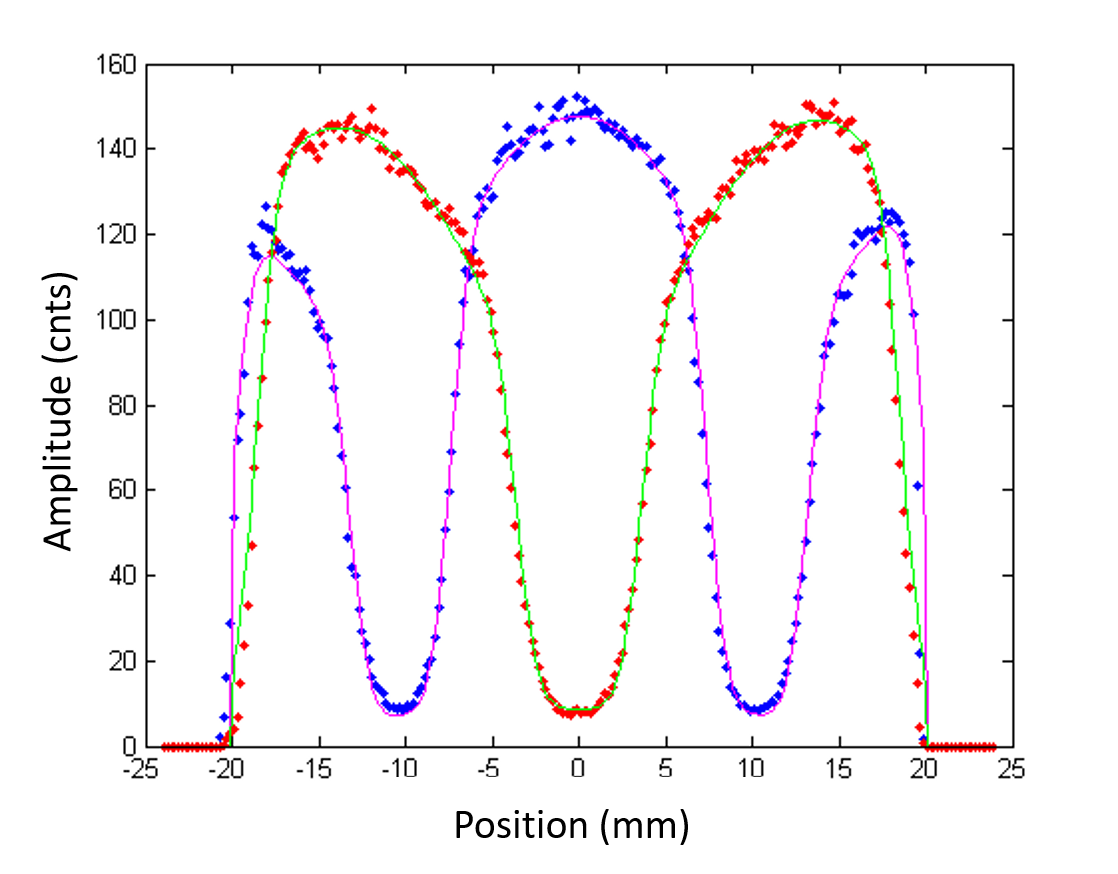
\includegraphics[width=2.9in]{figures/sns_prof.png}

The sensitivity calibration resulted in 20 planar projections; giving a measure of count variation for each detector. By inspecting a slice through the data with the sensitivity model a series of sensitivity profiles. Fig. \ref{fig_sensprof} shows examples of sensitivity profiles for two different collimator sections and the corresponding fits. This models were fitted for every slit section across the length of the collimator. Through the model a measure of count variation was determined and compared against the expected geometry of the system. Reconstruction was then corrected for the count variation for each slit section. 

\caption{Sensitivity profiles for two collimator sections and fitted analytical functions.}
\label{fig_sensprof}
%\vspace{-0.2cm}
\end{figure}

\section{Discussion}
The experiments carried out here were the first use of the calibration and acquisition procedures on the complete system. The goal of this study was to acquire the first phantom images and assess the system performance, however, we also look critically at the procedures and software used in the system. When compared to initial studies \cite{Michele} we found a degradation in system performance; this is due to ageing of the components and stress on the system from regular use. Despite this we were able to use the system extensively and collect a large quantity of data. The results of the investigation lead to changes in software, processing methods and calibration. 

The detector calibration revealed major issues when using the aged system. The channel instability resulted in data lost and false counts. The hot spots caused by faulty channels reduced the quality of the acquire data, requiring data channels to be removed completely from acquisition. Constant faulty channels could be switched off and accounted for with the \acrshort{LRF} models. Figure \ref{fig:killchan} demonstrates the corrections possible when using the adapted \acrshort{LRF} reconstruction. 

The \acrshort{LRF} is successful in accounting for faulty channels, however it is only effective when correcting for single channels. If several channels are missing in one place, there will not be enough neighbouring data to interpolate the missing area. When faced with large areas of detectors failure we can make use of dual acquisition. The two acquisition positions allow a larger area of data to be collected. By rotating the detector view we can retrieve angles from whole detector failure.

The linearity acquisitions made use of the BULMA software to produce correction maps. We found that large linearity distortion required manual intervention. This was time consuming as 40 data sets required manual correction. The acquisition of linearity data required individual scans which was also time consuming, combine these processes took 5 days to produce the linearity correction maps. As we have seen the stability of the detectors can lead failure in the calibration. In order to repeat the calibration regularly we require an improved process which can be done quickly and effectively.

The current software is only designed for the given calibration procedure. The software has out data which present truncated edges, which lose data and require image quality. In order to implement a new calibration procedure and remove the truncation issues we produced the construction of a new calibration software; chapter \ref{IEEE} will cover the implementation of this software. 

In following experiments we set out to change the system calibration procedures. The results of the geometric calibration were found to be constant; as the system geometry is fixed and known, we can calculate the parameters without calibration. The geometric calibration was designed for a single detector system and therefore no longer required in the complete system, we propose to remove this step in future investigations.

\section{Conclusion}
The calibration data was collected successfully and the results will be shown in chapter \ref{IEEE}. However the time taken to acquire and process this data was not acceptable for regular use. A new software and calibration process will be designed and implemented to improve use of the system. In the next chapter we will see how the phantom data is effected by the new software.

The stability of the system is a concern as faulty detectors and variability reduces the quality of the data. Although detector failure was accounted for, a further investigation is required to determine the extend of detector instability. The possibility of replacing faulty components would resolve many issues, until this time we continue to implement procedures to collect and process data quickly and  produce correct images.
 % calibration procedure and experimental method 
% Introduce need for new software NEW Event Recon and Lin Corr 
%\chapter{Linearity Software}
\label{chapterlabel}

% This just dumps some pseudolatin in so you can see some text in place.
\blindtext

\section{Introduction}

\section{Methods}

\section{Results}

\section{Discussion}

\section{Conclusion} % New methods for software and calibration 
\chapter{Phantom Images}
\label{IEEE}
% New Linearity and PERA software 
% Image comparison (Single, Dual, NEw software) 


\section{Introduction}
In this chapter, we outline the reconstruction of the phantom data acquired during our experiments at \acrshort{HSR}. The calibration and event reconstruction was carried out using the BULMA software as the software discussed in chapter \ref{Linearity} was yet to be completed. The series of phantoms shown in this chapter demonstrate the capabilities of the stand-alone \acrshort{SPECT} system and the procedures we can carry out to improve the quality of the images. 

\section{Image Reconstruction}
To successfully reconstruct the phantom data, all calibration corrections must be applied. Linearity and uniformity maps are applied directly to the planar data, whereas the geometric and sensitivity parameters are applied during reconstruction. The data are reconstructed using \acrshort{MLEM} \cite{4307558} in combination with angular blurring \cite{Bousse2013AngularReconstruction} \cite{8069508}. The system calibration determines how the event data are a product of collimator geometry.

\subsection{System Resolution}
The first set of phantoms we consider are the capillary acquired during geometric calibration. Figure \ref{fig:ImageRes} shows capillary phantom reconstructed and combined to give an image of all 60 sources. The image shows promising results across the \acrshort{FOV} as each capillary can be distinguished. We determined the system resolution by modelling the capillary images. The trans-axial resolution was determined at various radial positions across the detector's 20x20x9 $cm^3$ \acrshort{FOV}. A Gaussian model gave the radial and tangential resolution of each trans-axial capillary by the models \acrshort{FWHM}. There was a clear variation in \acrshort{FWHM} subject to position within the \acrshort{FOV}.

\subsection{Dual Reconstruction}
The reconstruction is limited by the angular sampling of the partial ring collimator. The introduction of a dual reconstruction of two sets of acquisition data allowed us to improve sampling angles. Dual acquisition is optional protocol which can be included in the system use. The phantom data may be acquired at two angular positions, separated by a rigid rotation about the z-axis. The second acquisition will provide projections from the missing region of the detector ring; an offset of half a detector also provides data in between each unit and provides improved angular sampling. 
\paragraph{}
The increased sampling overcomes detection failure over a large area; if a large region is missing, the rotated position can capture events from another detector unit. This improves sampling in the system as well correcting detector failure. The known positions of each acquisition are treated as two subsets, reconstructing both sets of data simultaneously, analogous to an \acrlong{OSEM} (\acrshort{OSEM}) algorithm \cite{Hudson1994AcceleratedData}. Each subsequent phantom was reconstructed with this dual method.

\subsection{Partial Volume correction} 
The images were further improved with the introduction of structural information. A simulated \acrshort{MR} acquisition from each phantom was used to determine the geometry and structural information. A post-reconstruction \acrlong{PVC} (\acrshort{PVC}) was carried out on the dual reconstructed image. The correction made use of the iterative Yang algorithm \cite{Erlandsson2012AOncology.}.

\section{Results}
 The results of modelling the capillary phantoms are shown in Fig. \ref{fig:resolution}. By combining the acquisitions we produced an image of 61 capillary sources spanning 5 radial positions. This image was used to determine the image resolution of the system subject to radial position. By modelling the capillaries in a the trans-axial plane with a 2D Gaussian, we determined the radial and tangential image resolutions. Measurements of the radial and tangential resolution show the effects of partial ring geometry; the bottom capillaries in Fig. \ref{fig:ImageRes} are in the region with no detectors and so the reconstructed values have a greater error. The system resolution is most stable closer to the centre of the \acrshort{FOV} where the partial ring effects are less prominent. The standard deviation in resolution is greatest on the edge of the FOV where the point sources appear to stretch radially, Table \ref{table_reso}.
  
\begin{figure}[!t]
%\vspace{-0.2cm}
\centering
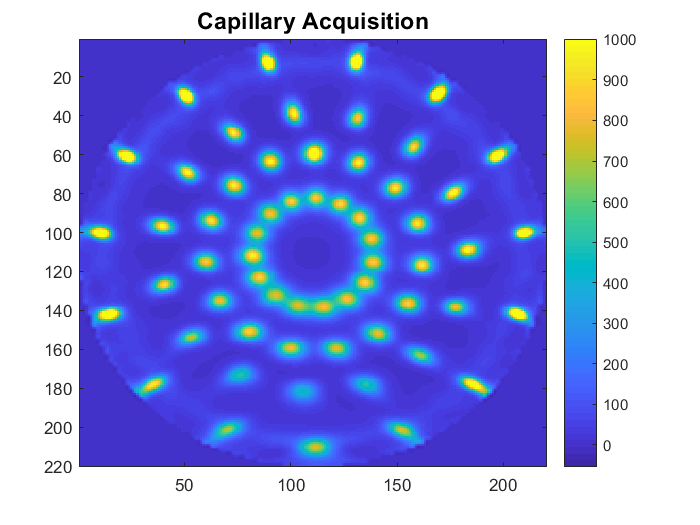
\includegraphics[width=4in]{figures/Capillary_newLRF}

\caption{The reconstructed capillary phantoms after corrections. The capillaries had 1mm diameter, each were filled with 10 MBq of $^{99m}Tc$ and were scanned for 5 minutes.}
\label{fig:ImageRes}
%\vspace{-0.2cm}
\end{figure}

\begin{figure}[!t]
%\vspace{-0.2cm}
\centering
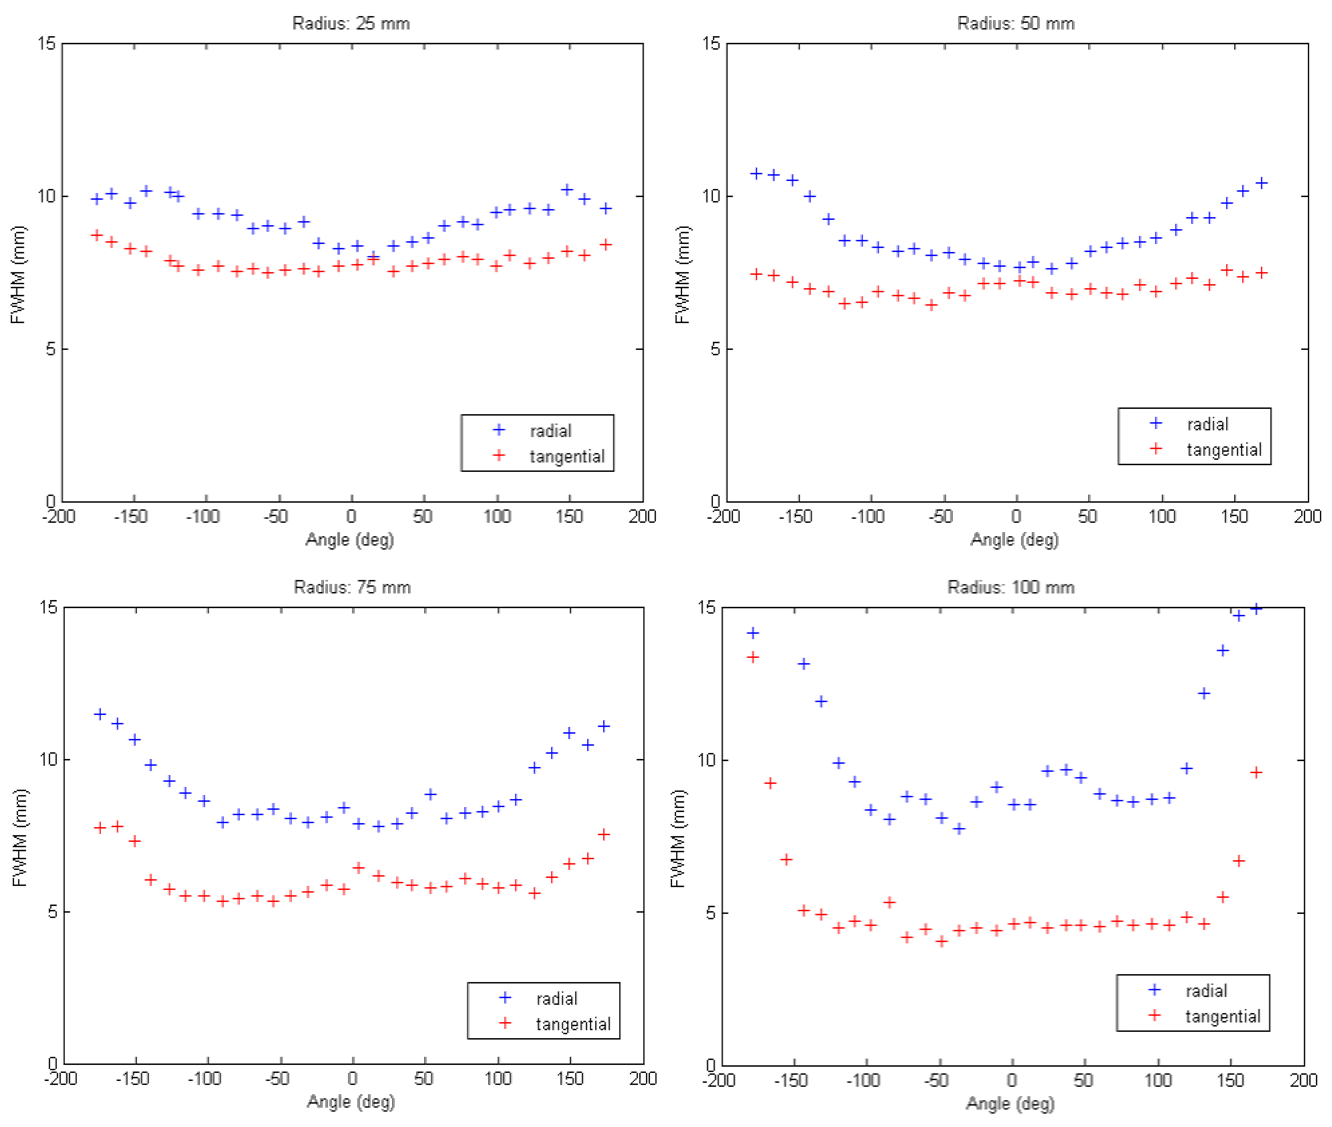
\includegraphics[width=5in]{figures/resolutions.png}

\caption{Resolution of capillaries at 4 radial positions against the angular position in the \acrshort{FOV}}
\label{fig:resolution}
%\vspace{-0.2cm}
\end{figure}

\begin{table}[!b]
% increase table row spacing, adjust to taste
\renewcommand{\arraystretch}{1.3}

\captionsetup{font=small}
\caption{Trans-axial Resolution}
\label{table_reso}
\centering

\begin{tabular}{|p{2.9cm}|p{4.6cm}|p{4.8cm}|}
\hline
Radial Position [mm]& Mean Radial Resolution [mm]& Mean Tangential Resolution [mm] \\
\hline
 25 & 9.39 $\pm$ 0.66 & 7.95 $\pm$ 0.51\\
\hline
 50 & 8.87 $\pm$ 1.15 & 7.31 $\pm$ 0.25\\
\hline
 75 & 9.49 $\pm$ 1.27 & 6.59 $\pm$ 0.95\\
\hline
 100 & 8.83 $\pm$ 2.00 & 5.1629 $\pm$ 1.08\\
\hline
\end{tabular}
\end{table}

 The phantom acquisitions include a Cold Rods phantom, a Hot Spheres phantoms and a 2D Hoffman Brain phantom. Figures, \ref{fig:cold}, \ref{fig:Hot} and \ref{fig:Hoffman}, show the results of the dual reconstruction method and the improvement from the post-reconstruction PVC.

\begin{figure}[!t]
%\vspace{-0.2cm}
\centering
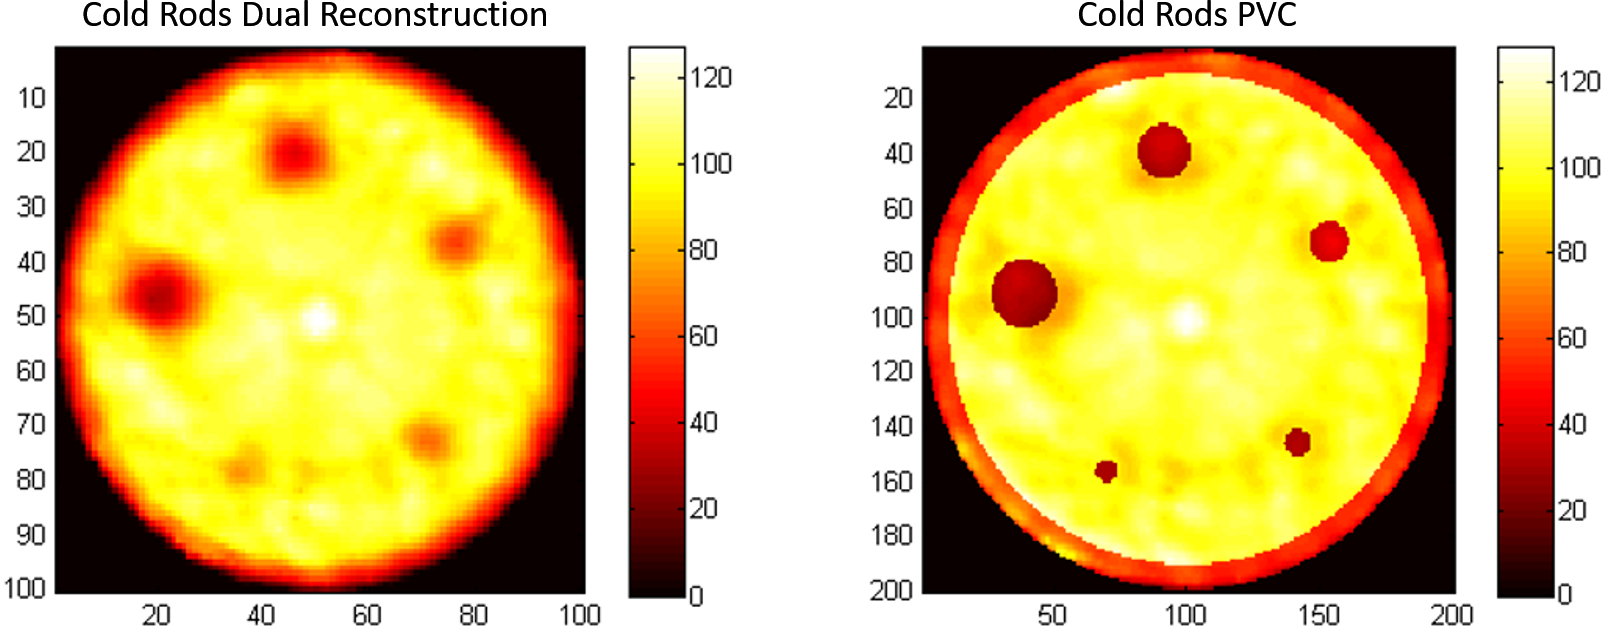
\includegraphics[width=4in]{figures/ColdRods.png}

\caption{Cylinder phantom of 50 MBq of activity and cold rods of diameters 8, 10, 15, 20 and 25 mm.}
\label{fig:cold}
%\vspace{-0.2cm}
\end{figure}

\begin{figure}[!t]
%\vspace{-0.2cm}
\centering
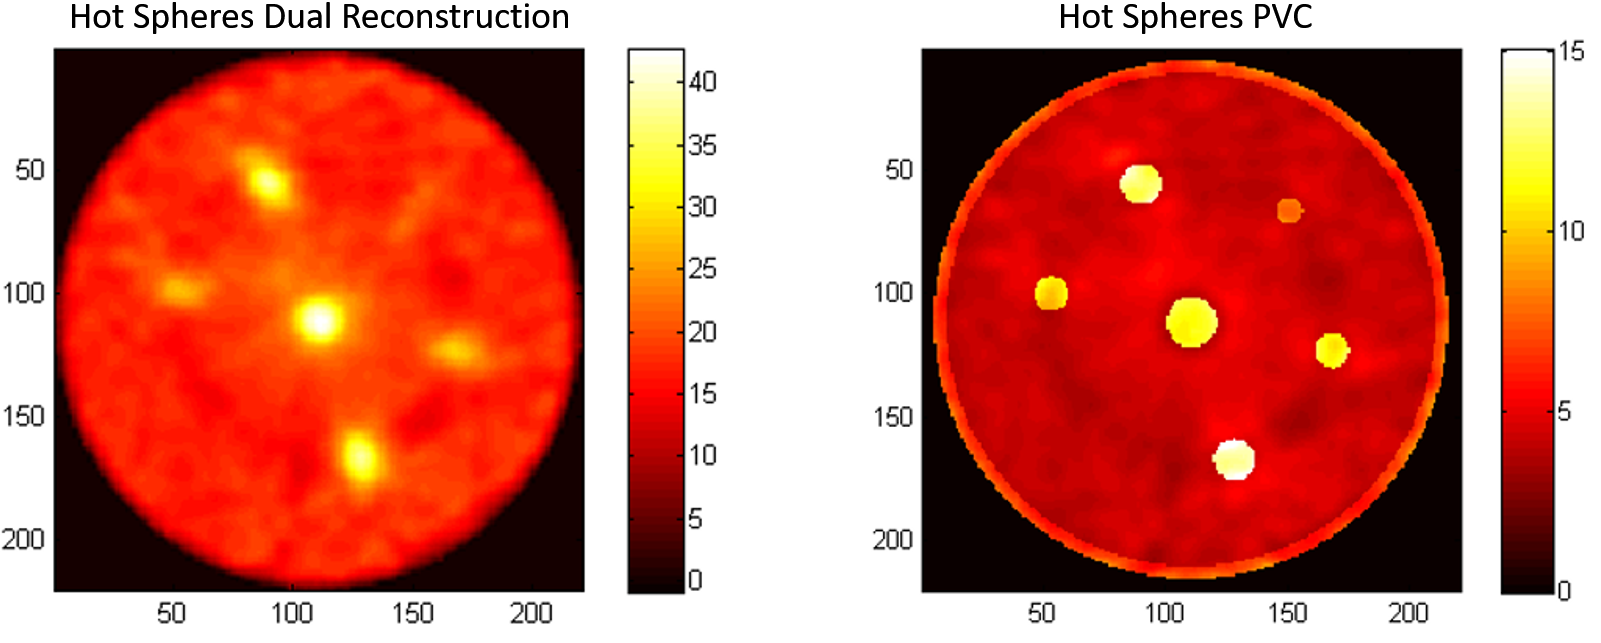
\includegraphics[width=4in]{figures/HotSpheres.png}

\caption{60 MBq to a ratio of 8:1 in the hot spheres of diameters 11, 14, 17, and 21 mm.}
\label{fig:Hot}
%\vspace{-0.2cm}
\end{figure}

\begin{figure}[!t]
%\vspace{-0.2cm}
\centering
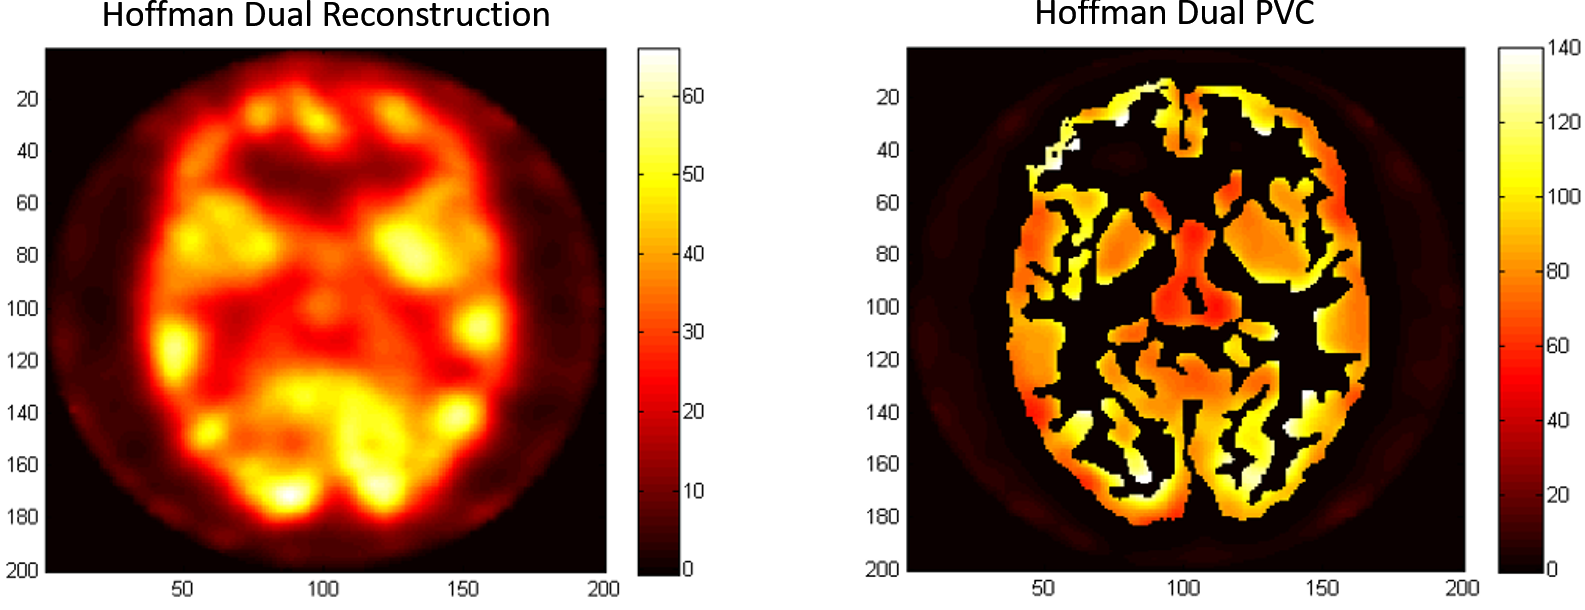
\includegraphics[width=4in]{figures/Hoffman.png}

\caption{2D Hoffman phantom with activity 25 MBq.}
\label{fig:Hoffman}
%\vspace{-0.2cm}
\end{figure}

\section{Conclusion}
The results from these phantom reconstructions show promising final images from the tabletop \acrshort{SPECT} system. The system shows signs of degradation as the results are worsened compared to previous studies and the intended design specifications. However, the age of the detectors is a likely factor in their degradation and instability \cite{Carminati2019ClinicalCharacterization}. 
\paragraph{}
We have demonstrated that the performance can be improved with a change in acquisition protocol. Implementing the dual reconstruction has shown to improve the images by improving angular sampling and compensating for faulty acquisitions. However we treat this as an extension to our system, the system is able to function and produce good quality images without this dual acquisition.
\paragraph{}
The inclusion of \acrshort{PVC} demonstrated the potential of incorporating \acrshort{MRI} data with the \acrshort{SPECT}. However, we must reproduce these reconstructions with real \acrshort{MRI} data to verify the results. 
\paragraph{}
The image quality is strongly related to the stability of the system and the accuracy of the calibration data. It is therefore essential to carry out regular calibration and keep track of the detector stability. Further experiments will set out to improve the image quality and detector stability by incorporating new calibration and acquisition procedures. 

\subsection{Discussion}
Overall the acquisition and reconstruction methods have demonstrated effective means of generating reconstructed images from incomplete data acquisition. We can correct for inhomogeneity and pixel failure in the detectors and produce correct projection data. The results of this research improved the processing of \acrshort{INSERT} projection data and introduced dual reconstruction, which can be used to benefit the system's clinical performance. We have determined a set of corrects which can be applied to the BULMA software to aid in the reconstruction of phantom data. 
\paragraph{}
However,  the instability of the system required further investigation. We are unable to adapt the BULMA software to account for detector failure and new calibration procedures. The implementation of adaptable software will allow us to incorporate further corrects to our data and develop a calibration procedure which can be carried out quickly and effectively. 
\paragraph{}
The \acrshort{INSERT} has undergone preliminary characterisation of the \acrshort{SPECT} system, however, complete \acrshort{MR} compatibility has only been validated in the preclinical system. Future work will set out to test the system in a clinical \acrshort{MR} environment and to streamline calibration and acquisition procedures for routine use. The use of \acrshort{MR} data will improve the images further and demonstrate the potential of the fully operational system.   

 % image reconstruction of experimental data with New method to compare 
%\chapter{Experiments 02}
\label{chapterlabel}


\section{Introduction}
The new system was tested with a second set of phantoms. The original calibration procedure was carried out here but the data was processed with the new software methods.
\section{Methods}

\section{Results}

\section{Discussion}

\section{Conclusion} % new data with new methods 
\chapter{Clinical Comparison}
\label{ClinicalComp}

% Clinical comparison with SPECT 
% MR compatibility 
% CLinical Installation 
% SPECT MR study 

Milan experiments revealed need for a smoother system and so a trolley was designed for the use of the scanner to aid loading. The uniformity flood was not carried out daily due to weight constraints which are not overcome with this design. 

\section{Introduction}
The final goal of this project is to establish clinical use of the first simultaneous \acrshort{SPECT} MRI system. In order to achieve this we must determine how the INSERT compares to existing SPECT systems and how the combination of SPECT and MR data can provide superior clinical information. 
\section{Methods}
The INSERT has been tested with a number of phantoms; to test the systems imaging capabilities against a standard clinical SPECT a complex phantom was used. An Aldersson Phantom was filled with ... $^{99m}Tc$ and scanned in several position in the INSERT system. The phantom scan was repeated in a ... clinical SPECT system.  
\section{Results}

\section{Discussion}

\section{Conclusion} % Future work Clinical comparison and steps toward clinic (trolley) 
\chapter{SIMIND}
\label{SIMIND}

% future experiments 
% Lin/Uni stability (phys)
% Lin Degree of distortion (sim)  
% Temperature effects  (phys)
% Alternative Calibration (both)
% Alternative design (sim) 


\section{Introduction}

SIMIND is a Monte Carlo software developed to simulate clinical Single Photon Emission Tomography (SPECT) systems. The software provides the design for standard clinical simulations, but also allows for the diverse modification of any experimental set up. Here we have implemented a new SPECT system, complete with a novel collimator design. The INSERT scanner is designed for the clinical SPECT acquisition of brain tumours. This system is a stationary, partial ring detector, designed to be a compact and Magnetic Resonance (MR) compatible. The multimini slit-slat (MSS) collimator is a novel design integral to the SPECT insert. This complete clinical system has been implemented in the SIMIND software and initial testing has been carried out here. 

The INSERT project has designed a complete clinical SPECT scanning system, intended for integration with standard Magnetic Resonance Imaging (MRI) systems. This design requires a stationary ring of compact CsI:Tl detectors, with Silicon Photomultiplier (SiPM) readout. The system design has previously been supported by Monte Carlo software, however here for the first time it is designed and tested in SIMIND. SIMIND provides a fast and diverse method of testing a novel system design, providing data to validate experiments and verify data acquisition.

In this work we outline a set of standard experiments carried out with the INSERT system. A set of phantom acquisitions were simulated, using the standard SPECT set up within SIMIND, along with the novel geometry of the MSS partial ring collimator. The data acquired from these experiments are used to verify a set of experiments carried out on the physical system. 

\section{Methods}
The novel system is defined within the SIMIND environment through a set of geometry files. These define the collimator design, detector specifications, and detector rotation and placement (spanning the partial ring). The experiments carried out involved the standard phantom set up available in SIMIND. Recreating our physical acquisitions, we simulated; capillary, cylindrical, planar, and Jaszczak phantoms. 

The projections acquired were reconstructed with Maximum Likelihood Estimation Maximisation (MLEM) algorithms, accounting for the system geometry by modelling the collimator resolution. The system properties were determined with the use of the capillary sources. The resulting phantom images were compared with that of the physical system.  

\section{Results}

\section{Discussion}

\section{Conclusion} % evaluation of calibration and system eval experiments and alternative system design 
% MILAN work with DOI and Energy and further corrections ect 
\chapter{Future Work}
\label{Future}

% LONDON install and experiments
%  MMR install
% CLinical comparison 
% SPECT MR study 
% NEW calibration procedure 
% Image Registration 
% SIMIND 
% Alternative Hardware 
% Alt. Use (Epilepsy, Foot, Bedside SPECT, cheap system ) 


% Clinical comparison with SPECT 
% MR compatibility 
% CLinical Installation 
% SPECT MR study 
Here we outline the future work set out to achieve the main goal of the project; the first in man study of \acrshort{SPECT/MRI}. However as this is a novel system there are many procedures to carry out to ensure the safe and effective use of the technology within the clinic.
\section{Calibration Technique}
As explained in previous chapters, the current calibration procedure procedure is impractical for regular use. The need for consistent calibration is clear from the instability of the system, and so we must reduce the time taken to carry out the calibration protocol. Due to a design oversight the linearity collimators are not \acrshort{MR} compatible; imposing further need for a calibration independent of these collimators. As the new calibration software has been implemented on existing data, we now have a versatile tool for producing calibration correction maps from alternative data set. The software can be amended to measure linearity from any linear source; allowing the linearity collimators to be removed from the protocol. 

The potential alternative linearity calibration would involve the use of a capillary phantoms. This technique would be similar to the geometrical calibration, where the \acrshort{MSS} collimator is used when acquiring a series of horizontal and vertical capillaries. The geometric and linearity calibration both involve a geometric transformation, carrying out these transformations simultaneously would be possible as the geometric distortion is minimal. The projects acquired from these phantoms would present of a series of linear lines which can be modelled with the new software. This technique would reduce the time needed to carry out a linearity calibration as multiple detectors can acquire data at a time. In order to carry out this technique within the \acrshort{MR} we would not be able to use the rotating motor, previously used to position the capillaries. An alternative would be to build a rotating frame or phantom to position the capillaries within the \acrshort{INSERT}  \acrshort{FOV}.

\section{SIMIND simulations}
Alternative procedures and designs, such as the calibration protocol, can be tested with Monte Carlo software. This would be a faster and cheaper method of testing proposed designed before they are implemented in the real system. 

SIMIND is a Monte Carlo software developed to simulate clinical imaging systems. The software provides the design for standard clinical simulations, but also allows for the diverse modification of any experimental set up. Michael Ljungberg developed SIMIND and has provided us with a prototype implementation of the clinical \acrshort{INSERT} scanner. This simulated environment would provide many possible experimental set ups and allow us to test proposed design changes with no risk to the physical system. 

The \acrshort{INSERT} has been simulated before to great success, however we moved to SIMIND as it promised a faster and more versatile software. The simulated \acrshort{INSERT} has not been fully tested and so future work with this system would require a complete implementation to ensure successful testing. 

\section{Clinical Studies}
To ensure the \acrshort{INSERT} is able to produce quality clinical \acrshort{SPECT} images we must compare it with existing technology. A phantom acquisition comparison of clinical \acrshort{SPECT} systems with the bench top \acrshort{INSERT} will allow us to assess the imaging capabilities of the INSERT. A phantom acquisition can be carried out using the standard procedures from both systems. The results will indicate how the \acrshort{INSERT} can be improved in order to measure up to clinical \acrshort{SPECT}.

As a patient study is the final goal of the \acrshort{INSERT} we must also be able to compare the results of our simultaneous \acrshort{SPECT/MR} to that of the current clinical procedures. As it stands the combination of \acrshort{SPECT} and \acrshort{MRI} data is only possible with a \acrshort{SPECT/CT} system. The \acrshort{CT} provides a common anatomical mapping with the \acrshort{MR} which can be registered onto the \acrshort{SPECT} data. Acquiring this data and carrying out the comparison will determine the effective use of the \acrshort{INSERT}. 

These studies will also enable the preparation of the first in man studies with the \acrshort{INSERT}. Achieving comparable results with clinical systems will help establish ethical approval for the use of the novel \acrshort{SPECT} technology. 

\section{Clinical installation}
Before we look to patient trials, it is essential that we prove the completed \acrshort{SPECT/MRI} system can function. The next immediate goal of this work is to carry out the installation of the \acrshort{INSERT} within a clinical \acrshort{MRI}. This task is a major challenge as we must be able to safely incoorporate each component of the \acrshort{INSERT} within the \acrshort{MR} environment. Following this installation we must carry out extensive tests to ensure the mutual compatibility of the \acrshort{SPECT} and \acrshort{MRI}. 

The installation of the \acrshort{INSERT} within the \acrshort{MR} have begun. We have installed the system within the Macmillan Cancer Centre's \acrshort{PET/MR}. This facility is designed for radiation safety and so makes the installation easier as we can integrate the \acrshort{SPECT} with existing nuclear medicine support. The \acrshort{INSERT} scanner is designed for \acrshort{MR} compatibility but the external components are not. The cooling system and electrical control boards are not suitable within the \acrshort{MR} and so must be controlled from outside. This has been considered and a series of filter plates have been designed to allow the control of the \acrshort{INSERT} from outside of the \acrshort{MR} room. The use of novel technology within the clinic requires health and safety considerations to ensure all risks are assessed with regards to the technology and users. With the help of the \acrshort{UCH} \acrshort{MR} team a standards of practise document has been created, which sets out the safe use of the \acrshort{INSERT} and considers the potential risks within the \acrshort{MR} environment. The document outlines the protocols which must be carried out, including the use of an \acrshort{MR} compatible trolley which has been designed specifically for the \acrshort{INSERT} scanner. Following our initial use of the scanner we established a need for an ergonomic collimator loading system, the trolley has been designed and built to ease the loading of the \acrshort{INSERT} and provide the safe use within the \acrshort{MR}. 

\include{Appendices} 
% You could separate these out into different files if you have
%  particularly large appendices.

% Actually generates your bibliography. The fact that \include is 
% the last thing before this ensures that it is on a clear page.
\bibliography{Bib/example}

% All done. \o/
\end{document}
